% Chapter 1--Introduction

\chapter{Architecture}
%%%%%%%%%%%%%%%%%%%%%%%%%%%%%%%%%%%%%%%%%%%%%%%%%%%%%%%%%%%%%%%%%%%%%%%%%
\section{The server}

The BlakSton server is designed to be a generic large-n world game
server which could potentially be used for several different online
games.  Keeping most game-specific code out of the server has made it
possible to make a robust server which has not crashed since the
system has been commercially available (as of this writing).

In order to make the server incredibly safe, I would estimate that
over half of the code is for error checking.  For example, even though
all Blakod objects' references to other objects are always valid, the
return value of \texttt{GetObjectByID} is checked against NULL.
Instead of using the now-common practice of using assertions to abort
a program when unforeseen circumstances arise, the server treats these
as possible error conditions and logs the problem, instead of
aborting.  Since even a single crash could cost hundreds or thousands
of dollars of customer service time, this was deemed crucial to the
game's success.

Since there is only a minimal amount of game-specific code in the
server, the overall design of the server is quite clean (and fairly
obvious).  The heart of the server is the Blakod interpreter, which
runs the actual game code.  Blakod calls are made when messages are
received from clients or timers expire.  Since the Blakod interpreter
is single threaded, only one call into Blakod exists at any time.
This puts several demands upon the interpreter.  First, it must be
rather fast, so that the server does not become backed up by client
requests.  Second, it must endeavor to prevent infinite loops or
infinite recursion in Blakod so that one poorly written Blakod
function does not hang the entire system.

To support the Blakod interpreter, the server has modules that handle
the storage of Blakod objects, Blakod list nodes, Blakod strings,
Blakod resources, Blakod strings, Blakod timers, and callback
functions.  These callback functions, called C code functions, exist
so that Blakod may interact with the server, since Blakod has no
inherent input or output.

The server's primary task outside of Blakod interpreting is keeping
track of network connections made by clients.  It needs to verify user
logins, allow administration of the game, and parse client messages
from the network to send the necessary messages to Blakod.

Client logins are mapped to accounts stored on the server.  Each different
physical person has his/her own account on the server, which they access
by logging in with their own account name and password.  Internally, the
server stores a unique account number for each account.  Each time an account
is created, it is given a new account number one greater than the previous
largest account number.  When an account is deleted, the account number
is no longer in use, and unless it was previously the largest account number,
is not reused.  Since account numbers are 32 bit integers, there is little
chance of them ever rolling over.

The server also keeps a map between account numbers and user objects in
the game.  Each account may have more than one user object mapped to it.
When a client requests that it would like to enter the game, the server
sends it a list of user objects which it may choose from.  This gives
the user the option of using any of their available characters in the game
each time he/she logs in.

The server maintains and controls all of the state associated with
avatar objects.  This information is all stored in the Blakod
properties of the object.  The client knows the avatar's position,
associated bitmap files, and a set of properties called ``object
flags''.  These flags are used to indicate that the client should
display the avatar with special effects, such as invisibility, color
translations, or shadowform.  The client also knows if the player is
paralyzed or resting, so that it can prevent user motion and running,
respectively, without a network round trip to the server.  The client
updates the server's knowledge of a player's position at most once a
second, to reduce server CPU usage.

\subsection{Network interface and threads}

The BlakSton Server communicates with other computers using TCP/IP
through the WinSock 1.1 interface.  WinSock 2 implementations are only
now available, and it is not known what benefits the server could
derive from using the new WinSock standard.

The server has two threads of execution.  The primary thread performs
nearly all tasks, including interpreting blakod and parsing messages
from clients.  The second thread is the interface thread.  It runs the
window interface and also performs asynchronous input/output on the
sockets that the server uses to communicate to clients.  The
programming overhead of using semaphores to lock access to the
server's buffers for client communication is onerous and difficult to
maintain.  However, it has proven successful.  Each time that any
thread needs to access either the input or output thread for a socket,
it first gets access to the buffer's semaphore, waiting for it
to be available if the other thread holds it.  The code then
reads or writes data from or to the buffer, and then releases the semaphore.
This is a standard way for multiple threads in a process to share
memory.

The interface thread is quite simple.  There is a main loop that
dispatches all Window events to the appropriate handler functions.
There are several GUI events that are used to provide simple ways to
save the game, terminate the server, and bring up an outdated help
system.  Also, the administrator commands sent by the GUI are passed
to the main thread to be handled there.

The only other events that the interface thread receives are events
pertaining to sockets.  The three different messages are sent when
bytes are received, the internal WinSock outgoing buffer changes from
a full to a non-full state, or the socket is closed.

When the interface thread receives bytes on a socket, it reads those
bytes and adds them to a queue for the appropriate session.  A session
is a data structure maintained by the server for each connected
client.  It includes input and output data queues, the session state
(whether the client is just logging in, is at the main menu, or in the
game), as well as the client's IP address, CPU type, and screen size.

After the bytes are added to the appropriate session's queue, the main
thread is signalled.  The main thread, when it receives a time
quantum, examines each session's queue and proceeds to parse new bytes
in each queue.

When the interface thread is notified that a socket's WinSock outgoing
queue is no longer full, it looks in the server's outgoing queue for
that session.  If there are bytes waiting to be sent, then the
interface thread immediately sends the queued bytes over the socket
and resets the queue.

When the interface thread is notified that a socket has been closed,
then the main thread is sent a message to close the appropriate
session and free any memory allocated for the session.

\subsection{Event handling}

The previous section describes the window events handled by the interface
thread.  Here is a description of the events sent to the main thread:

\begin{description}
\item[WM\_BLAK\_MAIN\_READ] The interface thread sends this when it reads
bytes from a client; the main thread responds to this message by parsing
the message if it is complete and sending the data to Blakod if necessary.

\item[WM\_BLAK\_MAIN\_RECALIBRATE] Sent by the main thread when the timer
node in the front of the timer node list changes, so we can reset the
time we'll wait for an event.  This is only an issue if a new timer is 
created that is set to go off before any other timer in the system.

\item[WM\_BLAK\_MAIN\_DELETE\_ACCOUNT] Sent by the main thread when an
administrator deletes an account.  We handle this by deleting the account.

\item[WM\_BLAK\_MAIN\_VERIFIED\_LOGIN] Sent by the main thread when
the billing system signals a valid login.  The appropriate session is then logged in.

\item[WM\_BLAK\_MAIN\_ALLOW\_LOGINS] Send by the main thread when
the billing system is enabled and has finished its initialization.  We respond
by calling \texttt{accept} on a socket to begin to allow client logins.

\end{description}

\subsection{Communication buffers}

Although WinSock has internal input and output buffers for each socket, I
chose to implement an additional level of buffering in BlakServ itself.  This allows
the server to theoretically read and write any length messages, no matter their
length, because the server buffers are implemented as a list of buffers.  This
has not been exploited, but is available.

The buffering system in the server is quite simple.  A session buffer list is
a singly linked list of \texttt{buffer\_node} structures, which contains a pointer
to a block to send (up to 5000 bytes in length), the actual length of the block,
and a pointer to the next node in the list.

To send bytes to a client session, the server calls a function called
\texttt{SendBytes} with the session structure, buffer, and buffer size to
send to the session.  \texttt{SendBytes} checks to see if the session already has
a send buffer list.  If the session is backed up, then the new block of bytes is
added to the end of the buffer list, and if necessary allocating new buffers on 
the end of the list.  If the session is not backed up, then the bytes are sent
straight to WinSock to send to the client.  If this call fails, then the bytes
are put in a buffer list and stored in the session structure.

Unlike transmitted data, all received data is always placed in a buffer list when
it is received by the interface thread.  The interface thread then sends a message
to the main thread that tells it to process the bytes in the appropriate session.


\subsection{Blakod interpreter}

When a complete message arrives from a client or a timer goes off, the
server sends a message to a Blakod object.  Client messages are always
sent to the Blakod object associated with the client's account, which
is always of the class \texttt{user} or descends from this class.  
Client messages can have up to 15
parameters.  Timer messages can be sent from the server to any object,
and have no parameters.

Parameters are actually referenced as local variables by the compiled
Blakod (called \emph{bkod}).  If a message gets passed $n$ parameters
and uses $m$ local variables, then then local variables $0..n-1$ are
actually parameters, and local variables $n..n+m$ are used as local
variables.

The core of the Blakod interpreter iterates through the bkod
instructions of one message handler.  Instructions can only modify
local variables for the message handler or properties of the object.
The only instructions that can communicate outside of the current
objects are CALL instructions, which invoke C code in the server.  A
complete list of the C functions is in the next section.

Some of the C code functions are quite simple, such as \texttt{Bound}
which is a combined min and max function.  However, most of the C code
functions are rather complex and do things that could not otherwise be
done in Blakod.  The most important may be \texttt{Send}.  This
function takes an object, a message name, and a set of parameter names
and values and invokes the Blakod interpreter on the destination
object with the given message and parameter values.  Since this is
implemented as a simple recursive call in the server, the original
call is suspended while the sub-call takes place.  Also, since the
server stack is used for this recursion, there is a check to make sure
that the recursion does not go on forever (such as in a Blakod
function that was infinitely recursive).  If the call stack gets too
deep, it is aborted and an error is printed in the error log.  If this
check did not exist, the server would crash.

The other two critical C code functions are \texttt{AddPacket} and
\texttt{SendPacket}.  These functions allow Blakod to build up a
packet of data and then send it over the network to a client.
\texttt{AddPacket} takes an even number of parameters; the odd number
parameters must be integers which specify the number of bytes of the
following parameter.  For example, since many player statistics are
known to be small, the protocol only allocates one byte for each
statistic.  So although object properties and local variables are
always four bytes, only the low one or two bytes are sometimes sent,
when the protocol calls for it.  \texttt{AddPacket} takes the values
and adds them to a global output buffer.  Once a full packet is built
up (from one or more \texttt{AddPacket} calls), the Blakod then calls
\texttt{SendPacket} along with a session number so the server knows
which client to send the packet to.  The user object is sent this
session number each time a client logs in, and stores it for use in
calls to \texttt{SendPacket}.

\texttt{SendPacket} adds a header to the data packet, and checks the
output queue for the destination session.  If it is empty, the server
calls the WinSock send function to instantly send the data to the
client.  If this fails, it adds the packet to the server's output
queue for the session which the interface thread will send later, when
it gets a message from WinSock that the send buffer is no longer
empty.  If the server's output queue is already non-empty, the packet
is just added to the queue.

\subsubsection{Built in functions}

\begin{description}

\item[create] Takes a class.  Creates a new object of the specified class, and sends it 
the \texttt{Constructor} message.
\item[isclass] Takes two parameters, an object and a class.  Returns the 
integer 1 if the object is of the specified class or any of the class' descendants.

\item[getclass] Takes an object.  Returns the class of the specified object.

\item[send] Takes an object, a message, and any number of parameters.  
Immediately sends the given message to the given object, with all of the specified parameters.
\item[post] Takes an object, a message, and any number of parameters.
Queues up the message in the Blakod message queue.  See the next section.

\item[debug] Takes any number of parameters.
Prints all parameters to the debug log, which is on the BlakServ
interface and \texttt{debug.txt}.

\item[addpacket] Takes any number of pairs of parameters.  The odd numbered
parameters are the lengths to send of the even numbered parameters.  Adds
the specified data to a send buffer, which can be sent to a particular client
with \texttt{SendPacket}.

\item[sendpacket] Sends any buffered up bytes (added by \texttt{addpacket}) to
the given session.  The buffer is then cleared.

\item[sendcopypacket] Sends any buffered bytes to the given session, while leaving
the buffered up bytes in place to be sent again.
 
\item[clearpacket] Clears the buffer of bytes to send to a session (in essense,
it cancels any \texttt{addpacket} calls since the last \texttt{sendpacket}).

\item[getinactivetime] Takes a session id.  Returns an integer of the number
of seconds since the server has received bytes from the session's client.
   
\item[stringequal] Takes two parameters, both of which can be either strings
or resources.  Returns the integer 1 if the two parameters are different only
in capitalization and spacing; otherwise returns the integer 0.

\item[stringcontain] Takes two parameters, both of which can be either
strings or resources.  Returns the integer 1 if any substring of the first parameter 
differs only in capitalization and spacing from the second parameter; otherwise
returns the integer 0.

\item[setresource] Takes a dynamic resource (a player's name) and a resource.  Sets
the dynamic resource to the string value of the resource.

\item[parsestring] Takes a string, a debug string (string contained in quotes
in Blakod source code), and a message.  Calls the C runtime function \texttt{strtok}
on the string using the debug string as separators, and calls back the calling
object with the specified message for each parsed string.  Only used for parsing
the destination field of mail messages.

\item[setstring] Takes a string and a resource.  Sets the string to the string
value of the resource.

\item[createstring] Returns a new, zero length string.

\item[createtimer] Takes an object, a message, and an integer number of milliseconds.
Adds a node to the timer queue to call the specified message on the specified object
in the specified amount of time.  Returns the timer id, which can be used in calls
to \texttt{deletetimer} and \texttt{gettimeremaining}.

\item[deletetimer] Takes a timer id.  Removes the timer from the timer queue.

\item[gettimeremaining] Takes a timer id.  Returns the integer number of milliseconds
before the specified timer is set to go off.

\item[createroomdata] Takes a resource, which must specify the filename of a room
file.  Loads the server movement grid in the specified room file and returns a
room id, which as an integer that is different from the room id of any other loaded room.

\item[roomdata] Takes a room id.  Returns a list of length 3 containing the 
grid row size of the room, the grid column size of the room, and the security
number of the room.

\item[canmoveinroom] Takes a room id, a source row and column, and a destination
row and column.  The destination row and column must specify a square that directly
neighbors the source square.  Using the server movement grid of the specified room,
returns 1 if an object is able to move from the source row and column to the destination
row and column; otherwise returns 0.

\item[cons] Takes two parameters; the first can be any value, the second must be a 
list.  Adds the first element to the beginning of the list, by creating a new list
node.

\item[first] Takes a list.  Returns the first element of the list.

\item[rest] Takes a list.  Returns the list without its first element.

\item[length] Takes a list.  Returns the length of the list.  A nil list has
length zero.

\item[nth] Takes a list and an integer (call it $n$).  Returns the $n$th element
of the list.

\item[list] Takes two parameters.  Returns a two element list, whose first element
is the first parameter and second element is the second parameter.

\item[islist] Takes one parameter.  Returns 1 if the parameter is a list; otherwise
returns 0.

\item[setfirst] Takes a list and any value.  Sets the first element of the list
to be the specified value.

\item[setnth] Takes a list, an integer (call it $n$), and any value.  Sets the
$n$th element of the list to be the specified value.

\item[dellistelem] Takes a list and any value.  Returns the list with the first
occurrence of the specified value removed from the list.

\item[gettime] Returns the number of seconds since January 1st, 1996.

\item[abs] Takes one integer.  Returns the absolute value of the integer.

\item[bound] Takes an integer (call it $n$) and two values which can be integers or nil.  
Call the first of these $a$ and the second $b$.  If $a$ and $b$ are both nil, then this
function returns $n$.  If $a$ is nil and $b$ is an integer, then it returns min($n$,$b$).
If $a$ is an integer and $b$ is nil, then it returns max($n$,$a$).  If both $a$ and $b$
are integers, returns min(max($n$,$a$),$b$).

\item[createtable] Creates a new hash table with 2999 available entries.  Returns a table
id which uniquely identifies the newly created hash table.

\item[addtableentry] Takes a table id, a key value, and a data value.  Using the
hash function from the ELF file format, calculates the hash value of the key and
inserts the key value and data value into the table using open hashing.

\item[gettableentry] Takes a table id and a key value.  Returns the data value
associated with the key value from the specified table.

\item[deletetableentry] Takes a table id and a key value.  Deletes the data value
associated with the key value from the specified table.

\item[deletetable] Takes a table id.  Deletes the entire table.
   
\item[random] Takes two integers.  Returns an integer randomly chosen from the closed
interval defined by the two integers.

\end{description}

\subsubsection{Objects}

The most important data in BlakServ are Blakod objects.  They are stored in one large,
dynamically sized array of the following structure:
\begin{verbatim}
typedef struct
{
   int object_id;
   int class_id;
   Bool deleted;
   int garbage_ref;
   int num_props;
   prop_type *p;
} object_node;
\end{verbatim}

Here is what each element of the object node structure means:

\begin{description}
\item[object\_id] This value is the same as the object's index in the object array.
\item[class\_id] This specifies the class of the object.
\item[deleted] This is used by the garbage collector to keep track of which
objects are not referenced and need to be deleted.
\item[garbage\_ref] This is used by the garbage collector to store what this object's
new object id will be after the garbage collection is done.
\item[num\_props] This is the number of properties used by this object.
\item[p] This is the actual array of property values for this object.
\end{description}

Initially the array is allocated to store ten thousand objects.  However, as the game
runs, objects are created, using up this space.  Over time, ten thousand objects
may not be able to hold every object.  In this case, the array is reallocated
at twice its previous size.  This means that the array is never ``full'', because
even if there are no open entries, it will automatically be resized to store more
objects.

\subsubsection{List nodes}

Another key part of Blakod is list nodes.  Although they act much like
LISP lists, all operations are destructive--the server itself never
makes a copy of changed list.  This reduces memory usage considerably,
but requires more care on the Blakod programmer's part.  They are stored
in one large, dynamically sized array of the following structure:
\begin{verbatim}
typedef struct
{
   val_type first;
   val_type rest;
   int garbage_ref;
} list_node;
\end{verbatim}

Here is what each element of the list node structure means:

\begin{description}
\item[first] This is a Blakod value (4 bits tag, 28 bits data) of the
current node in the list.
\item[rest] This is a Blakod value of the next node in the list (or nil
if it is the end of list).  If this is not nil or a list node, then
it works exactly like dotted pairs in LISP.
\item[garbage\_ref] This is used by the garbage collector to store what this
list node's new list node id will be after the garbage collection is done.
\end{description}

\subsubsection{Resources}

Resources are a simple construct used to prevent the server from having to
send the actual text of preprogrammed strings over the network every time
they are used.  They are defined in the resource section of a Blakod source
file, and stored in the server in a linked list of the following structure:
\begin{verbatim}
typedef struct resource_struct
{
   int resource_id;
   char *resource_val;
   char *resource_name;
   struct resource_struct *next;
} resource_node;
\end{verbatim}

Here is what each element of the resource node structure means:

\begin{description}
\item[resource\_id] The number assigned to this resource string by the
Blakod compiler.
\item[resource\_val] The string which defines this resource.
\item[resource\_name] The name of the string, which is used in Blakod
to reference the resource.
\item[next] A pointer to the next resource node in the linked list.
\end{description}

\subsubsection{Strings}

Blakod uses strings to represent text data that can change--anything not
written by the development team.  For example, player descriptions are
stored as strings.  All player speech is stored as strings, although
they use one special string (called the \textit{temp string}) to reduce
memory allocations.  No strings are created by the Blakod (except by the
chess game to store its state).  They are parsed from client messages and
passed into the Blakod.  They are stored in the server as a dynamically sized
array of the following structure:
\begin{verbatim}
typedef struct
{
   char *data;
   int len_data;
   int garbage_ref;
} string_node;
\end{verbatim}

Here is what each element of the string node structure means:

\begin{description}
\item[data] The actual bytes of the string (in ASCII).
\item[len\_data] The length of the string.
\item[garbage\_ref] This is used by the garbage collector to store what
this string node's string id will be after the garbage collection is done.
\end{description}

\subsubsection{Blakod timers}

Blakod timers play a large part in programming any game based on the BlakSton system.
They are stored in a linked list, sorted by the time they are set to go off (the next
timer to go off is first in the list).  The linked list is composed of the following
structure:
\begin{verbatim}
typedef struct timer_struct
{
   int timer_id;
   int object_id;
   int message_id;
   unsigned int time;
   int garbage_ref;
   struct timer_struct *next;
} timer_node;
\end{verbatim}

Here is what each element of the timer structure means:

\begin{description}
\item[timer\_id] This is a number which is unique among all the timers and can be 
referenced from Blakod to get the remaining time on this timer or to delete it.

\item[object\_id] This is the object that will be sent a message when the timer goes off.

\item[message\_id] This is the message that will be sent to the object when the timer
goes off.

\item[time] This is the time the timer will go off, measured in milliseconds since
Windows started, and hence can be compared to the result of the Windows call
\texttt{timeGetTime()}.

\item[garbage\_ref] This is used by the garbage collector to store what this timer's
new timer id will be after the garbage collection is done.

\item[next] This is a pointer to the next timer node in the linked list of Blakod timers.
\end{description}

Blakod can control timers with the \texttt{CreateTimer()}, \texttt{GetTimeRemaining()},
and \texttt{DeleteTimer()} calls, as described in the previous section.

The main loop of the server operates in the obvious way with Blakod timers.  At the
beginning of the loop, it checks the timer list to determine the amount of time until
the next timer is set to go off.  It then waits for events (network events sent 
by the interface thread) for up to that period of time.  If it receives no events,
it removes the timer from the timer list, and calls the specified Blakod object with
the specified message, which handles the timer.  After the Blakod call is returned,
the main loop starts again, calculating the next timer and waiting for an event.

\subsubsection{System timers}

BlakServ has a number of system timers, which are activated on a periodic basis.
Every time the main thread gets a network related message from the interface thread,
it checks to see if any system timers are ready to go off, and if so, performs 
the appropriate action.  Unlike Blakod timers, system timers are not created and
deleted.  They are created once when BlakServ starts, and are never deleted.  The
following list describes the various system timers (by their symbolic names used in
the server).

\begin{description}
\item[SYST\_GARBAGE] Performs garbage collection.
\item[SYST\_SAVE] Saves the state of the game to disk.
\item[SYST\_BLAKOD\_HOUR] Sends the system object a message saying that
a game hour has elapsed.
\item[SYST\_INTERFACE\_UPDATE] Sends a message to the interface thread to
update the statistics on the user interface.
\item[SYST\_RESET\_TRANSMITTED] Resets an internal count of the number of
bytes written to the network since the last time the count was reset.
\item[SYST\_RESET\_POOL] Frees buffers used by the network buffering system.
\item[SYST\_CHECK\_PORTAL] If the billing system to communicate billing information
to an outside program is enabled, this checks to make sure the TCP/IP socket
used for communication is still active.  If it is not, it attempts to
reconnect to the outside program.
\end{description}

\subsubsection{Blakod message queue}

The Blakod message queue is implemented by a small bit of code I wrote one afternoon
in March 1996.  The problem that we faced was quite disturbing--NPC characters
were responding to player speech before the speech was sent to everyone in the room!
What happened was that when a player sent a \texttt{BP\_SAY} message, the room object
send a \texttt{SomeoneSaid} message to every active object in the room.  If an NPC
was before a player in the room list, then it would see the speech and respond to it
to every active object in the room.  After this, the original text would then be sent
to the rest of the active objects in the room.

At that point, there was only one top-level message being interpreted at any time.  The
top-level message (called directly by the server) may send other messages, but when the
original top-level message returned, control returned to the server which returned
to the main loop.

To solve the speech problem, I created the Blakod message queue.  When the original
top-level message is sent, the queue is empty.  While the server is interpreting
Blakod, it can call \texttt{Post()} which adds an element to the Blakod message
queue.  When the top level message returns, the server enters a loop that
dequeues an element from the Blakod message queue and sends the indicated object
the appropriate message.  This is done until the queue is empty.

This solved the NPC speech problem nicely.  When an NPC gets a message from
a player that it wants to respond to, it posts itself a message, which gets
dealt with after all the players in the room hear the initial player speech.

The Blakod message queue is a queue of the following structure:
\begin{verbatim}
typedef struct
{
   int object_id;
   int message_id;
   int num_parms;
   parm_node parms[MAX_NAME_PARMS];
} post_node;
\end{verbatim}

\begin{description}
\item[object\_id] The object to send a message.
\item[message\_id] The message to send to the object.
\item[num\_parms] The number of parameters being sent.
\item[parms] The actual values of the parameters being sent.
\end{description}

\subsubsection{Garbage collection}

The garbage collection system exists in BlakServ to reclaim memory wasted by
objects, list nodes, and strings that are no longer needed in the game.  Without
garbage collection, any machine running BlakServ would run out of memory in
a matter of days.  With garbage collection, BlakServ is able to run for weeks at a
time without needing to be stopped and restarted.  

BlakServ uses the ``stop and sweep'' 
garbage collection strategy, which means
that for a fraction of a second the server stops all processing, performs
garbage collection, and then resumes normal operation.
Garbage collection is performed in several stages.  The first stage reclaims
list nodes, the second stage reclaims objects, and the final stage reclaims
strings.

The garbage collection system uses the \texttt{garbage\_ref} field of the various
structures as temporary storage to keep track of which structures are referenced
and what their new id will be after the garbage collection is done.  The list node
garbage collection starts by traversing every property of every object and marking
every list node referenced by a property.  Each list node that is referenced is
then given a new list node id in its \texttt{garbage\_ref} field.  All objects
are again traversed, and any references to list nodes are changed to refer to the
new list node's new id.  Then, the list node array itself is compacted, so that
unreferenced list nodes are deleted and all list nodes have their new list node
id.  One important thing to note about list node garbage collection is that there
is a flaw--objects that are later cleared in object node garbage collection may
reference list nodes and these list nodes will be saved, even though they could
be erased.

The garbage collection of objects works in a similar fashion.  It is slightly
complicated by the fact that objects are referenced by more places in the server
than list nodes.  Object node garbage collection begins by traversing the objects
associated with every user account in the system.  Every object referred to by a property
of a user object is marked as referenced and then recursively checked itself--any object
referred to by their properties is marked, etc.  If a property is a list node,
then the list is traversed and any objects referred to by the list are marked and
then checked themselves.  The system object is also automatically marked and traversed.
In this way, every object that is still used by the game is marked as needed, and all
unreferenced objects can be prepared to be deleted.  No Blakod messages are sent
during garbage collection to garbage collected objects.

The garbage collector next goes through every object and gives all marked objects
a new object id in the object's \texttt{garbage\_ref} field.  It then proceeds to
traverse every property of every object, every list node, user account, session,
and timer and replaces any object id with the new post-garbage collection object id.
Then, the object node array itself is compacted, so that unreferenced objects
are deleted and all object nodes have their new object node id.

String garbage collection works much the same way.  First, every property of every object
is traversed, and all strings that are referenced are marked.  All list nodes and
other objects referenced by each traversed property are recursively traversed,
thereby marking all strings referenced by any object or list node in the system.
Each marked string is then given a new string id which is temporarily stored in
each string node's \texttt{garbage\_ref} field.  Each object and list node is traversed
and all references to strings are changed to refer to the string's new post-garbage
collection id.  The string nodes are then traversed and non-referenced string nodes
are deleted.

Timer garbage collection works much the same way, although it is a bit simpler.  Timers
aren't garbage collected, because they are automatically deleted when they go off.  At
garbage collection time, each timer is given a new timer id.  The lowest id timer becomes
timer id 0, and each timer is given a new id one larger than the previous timer's id.  Then,
each object and list node is traversed and timer id's are changed to the new id.  This
allows timers to be freely used in Blakod without the fear that timer id's could rollover
28 bits and cause problems.

As described earlier, BlakServ was designed to be a very stable server.  In order
to prevent crashes, many checks are performed on function return values which
should be guaranteed.  For example, in the garbage collector, for every list
node that is attempted to be traversed, the list node id is checked to be valid.  
If a list node that is referenced does not exist, a ``death by garbage collection''
error is printed, and the server does not crash.  However, with a serious error
such as this, objects will be left with invalid references, which may cause
the game not to function, depending on the specific Blakod.  Checks are performed
on objects, list nodes, strings, and timers, and all could report an error.  Invalid
references can only exist if there is a serious bug in either Blakod or BlakServ.
Correct code will not generate these types of errors.



\subsubsection{Optimizations and bottlenecks}

Blakserv was designed to be limited in performance only by the CPU power of the
machine it runs on.  In other words, given any reasonable network connection
and any type of connections to client machines, the number of clients that
the server can handle at one time is limited only by the speed of the server CPU.
We believe that the server spends most of its time interpreting Blakod.  Therefore,
the obvious place to try to improve the server would be the Blakod interpreter.
This would give the best cost/benefit ratio of any work done to optimize the server.

I performed some profiling tests on the server in the summer of 1995 which allowed
me to increase the server performance by about 50\% on a Pentium class machine.
I achieved these gains by inlining the \texttt{RetrieveValue} function, changing
a linked list of all loaded Blakod classes into a hash table, and giving the class
structure a pointer to its parent class, rather than just the parent class id.

At this point in the evolution of Meridian 59, the Blakod interpreter is quite
efficient; I do not believe that much performance could be gained by changing
the server algorithms.  Rewriting the main interpreting loop in assembly might
give a reasonable boost in performance.  However, there is a large amount of Blakod
that has been written with little regard to performance.  Several performance
critical messages (those dealing with player motion) could most likely be analyzed 
and simplified to make the server able to handle more users. 

\subsubsection{State diagram}
The following diagram shows the possible states and state transitions for
each connected client.  The second diagram shows the substates and substate
transitions while in STATE\_GAME.  Note that STATE\_RESYNC, STATE\_TRYSYNC,
GAME\_BEACON, and GAME\_FINAL\_SYNC are not necessary since we communicate
with clients using TCP, a reliable protocol.  They exist because communication
over serial ports was supported for the first year the system existed, but
has since been removed.

\begin{picture}(300,500)(0,100)

\put(140,450){\framebox(120,40){STATE\_SYNCHED}}
\put(0,400){\framebox(120,40){STATE\_RESYNC}}
\put(0,330){\framebox(120,40){STATE\_TRYSYNC}}

\put(280,400){\framebox(120,40){STATE\_ADMIN}}

\put(140,270){\framebox(120,40){STATE\_GAME}}

\put(200,540){\vector(0,-1){50}}
\put(210,515){\makebox(0,0)[l]{New client connection}}

\put(140,470){\vector(-3,-1){88}}
\put(81,461){\makebox(0,0)[r]{Error parsing message}}

\put(60,400){\vector(0,-1){30}}
\put(50,390){\makebox(0,0)[r]{Beacon string}}
\put(50,380){\makebox(0,0)[r]{received from client}}

\put(120,370){\vector(1,4){20}}
\put(134,415){\makebox(0,0)[l]{Detect string}}
\put(131,405){\makebox(0,0)[l]{received}}
\put(128,393){\makebox(0,0)[l]{from client}}

\put(260,470){\vector(3,-1){88}}
\put(301,466){\makebox(0,0)[l]{BP\_REQ\_ADMIN received}}
\put(326,456){\makebox(0,0)[l]{from admin session}}

\put(280,440){\vector(-2,1){20}}
\put(270,445){\makebox(0,0)[tr]{\texttt{quit}}}	
\put(270,435){\makebox(0,0)[tr]{typed}}	

\put(207,450){\vector(0,-1){140}}
\put(210,330){\makebox(0,0)[l]{BP\_REQ\_GAME received from client}}

\put(125,120){\framebox(150,40){STATE\_MAINTENANCE}}
\put(210,210){\vector(0,-1){50}}
\put(220,190){\makebox(0,0)[l]{New connection on}}
\put(220,178){\makebox(0,0)[l]{maintenance port}}

\end{picture}

\subsubsection{STATE\_GAME Substates}
\begin{picture}(300,230)(0,70)

\put(190,200){\framebox(120,40){GAME\_NORMAL}}
\put(50,150){\framebox(120,40){GAME\_BEACON}}
\put(50,80){\framebox(120,40){GAME\_FINAL\_SYNC}}

\put(250,290){\vector(0,-1){50}}
\put(260,265){\makebox(0,0)[l]{Entering STATE\_GAME}}

\put(190,220){\vector(-3,-1){88}}
\put(131,211){\makebox(0,0)[r]{Error parsing message}}

\put(110,150){\vector(0,-1){30}}
\put(100,140){\makebox(0,0)[r]{Beacon string}}
\put(100,130){\makebox(0,0)[r]{received from client}}

\put(170,120){\vector(1,4){20}}
\put(184,165){\makebox(0,0)[l]{Detect string}}
\put(181,155){\makebox(0,0)[l]{received}}
\put(178,143){\makebox(0,0)[l]{from client}}


\end{picture}
\subsubsection{Memory usage}

The server allocates and frees a good deal of memory over the course of time.  These
allocations are tracked by a number of categories in order to track down memory 
leaks without too much effort.  Any administrator can see the current totals
with the admin command \texttt{show memory}.  Much more memory is used to store
the game objects and list nodes than anything else.

Here are the memory categories:

\begin{description}
\item[Timer] Blakod timer nodes.
\item[String] Blakod strings.
\item[Kodbase] The symbolic names of resources (read from kodbase.txt).
\item[Resource] The resource nodes themselves.
\item[Session] Session nodes.
\item[Account] User account information.
\item[User] User to game object mapping information.
\item[Motd] Message of the day.
\item[Dllist] DLlist nodes which store filenames to send to clients for updates.
\item[LoadBof] Nodes which point to loaded compiled Blakod.
\item[Systimer] System timer nodes.
\item[Nameid] Mappings of class ids and message ids to their Blakod names.
\item[Class] Class nodes for each Blakod class.
\item[Message] Message nodes for each message in each Blakod class.
\item[Object] Blakod object nodes.
\item[List] List nodes.
\item[Object properties] The properties of each Blakod object.
\item[Configuration] The hardcoded configuration options.
\item[SMTP] Memory used by current email account creation/deletion connections.
\item[Rooms] The movement grids of loaded room files.
\item[Admin constants] Name constants usable in admin mode.
\item[Buffers] Communication buffers.
\item[Game loading] Used while loading a saved game.
\item[Tables] Blakod hash tables.
\end{description}

%%%%%%%%%%%%%%%%%%%%%%%%%%%%%%%%%%%%%%%%%%%%%%%%%%%%%%%%%%%%%%%%%%%%%%%%%
\section{The client}

\subsection{Control flow and event handling}

As described in section~\ref{sec:modules}, the client has its own
internal message system that it uses to pass events to a set of {\em
modules}, or Windows DLLs.  In fact, when the client starts up, one of
the first things it does is load a module called {\tt intro.dll}.  In
the case of Meridian 59, this module displays a corporate logo and
then a splash screen for the game.  When the player clicks on a button
on the main window, the module unloads itself.

The client has a structured system for handling Windows messages.
Each incoming message is sent to a handler function, which then
dispatches the message according to the state the client is in.  The
state is a single variable that can assume one of several values (see
section~\ref{sec:clistate}).  Each state has an initialization
function that the client calls when it enters the state, and an exit
function that it calls when leaving the state.

Modules may call any of over 100 functions that the client exports to
them.  Thus, in many cases, control passes from Windows, to the
client, to a module, and then back to the client.  It is also possible
for modules to communicate with each other directly, although this
feature is not currently used.

The client can tell which objects are players via the object flags
that are associated with each object in protocol messages from the
server.  There is a bit reserved in the object flags bit vector that
indicates that an object is a player.  The client cannot tell which
objects are ``NPCs'' (a term without meaning in Blakod).  However,
object flags indicate which objects are attackable, and which are
legal targets of offer and buy commands; this usually distinguishes
animate objects from inanimate ones.

\subsubsection{Windows sockets}

When data is ready to be read from the socket connection to the
server, the client receives a Windows message.  The client then
retrieves all the available data and places it in a buffer.  Because
BlakSton uses TCP, boundaries between client/server messages may not
match boundaries between TCP segments.  Thus, the client checks to see
whether it has a complete protocol message each time it receives data
over the socket.  If so, the message is parsed and sent to an
appropriate handler function.  The client also handles cases where a
single TCP segment contains multiple protocol messages.

The call to open a socket connection to the server is done
asynchronously, so that the user can abort it if it takes too long.
However, the DNS lookup of the server's IP address is still done
synchronously.

\subsubsection{Keyboard handling}

The standard Windows keyboard messages are not really sufficient for
use in a serious game.  For one thing, key down messages aren't always
matched with a key up message because of dialog boxes appearing and
disappearing, and there is also a flaw in the reporting of key states
with the Num Lock key.  Therefore, when the client receives a key down
message, it begins polling the keyboard once per frame.  The state of
the entire keyboard is read, and special code gets around the Num Lock
problem.

The number pad keys generate different key code values depending on
whether the num lock toggle is on.  Due to an apparent bug in Windows,
when a key is pressed, num lock is toggled, and then the key is
released, the key up code is not always the same as the key down code.
The special num lock handling code synthesizes an up message for all
of the number pad keys whenever any key is released.  Without this,
the original number pad key would remain down, which causing the
player to spin out of control, since these keys are used for movement
and turning.

Each key, along with the state of each of the modifier keys (Shift,
Ctrl, Alt) may map to a user action.  The mapping of key states to
action is stored in key tables.  Each client game state has a list of key
tables associated with it, and calls exist for modules to add and
remove their own key tables.  Thus, the client itself doesn't contain
any information about the actions bound to keys.  The one exception is
the F1 key, which is bound to running the Web browser on the Meridian
help files.  This key is handled as a special case so that the F1 key
provides help anytime the client is running (not just when the client
is in the game state).

Some user actions, like moving and turning, can occur once per frame,
while most others should only repeat at a certain maximum rate.
Further, only one motion and one turning action should be allowed per
frame, so that players can't move faster by just holding down more
keys.  The keyboard handler handles move and turn actions differently
from other actions to account for these game play considerations.


\subsubsection{Animation}

When the client is the foreground application, it renders a frame each
time Windows notifies it that its event queue is empty.  This ensures
that rendering occurs at the fastest possible rate.  However, when the
user moves the client to the background, it makes sense to free some
CPU time for the new foreground task.  Windows also stops delivering
idle notification messages to the client when it moves to the
background, or (inconveniently) when a menu or dialog pops up.

To get around these problems, the client starts a timer when Windows
informs it that idle messages would no longer be delivered.  This
timer goes off ten times a second; when the client receives a timer
message, it renders a frame.  Thus, the game animates its 3D view at a
reasonable rate while allowing external programs to run with
reasonable performance on most machines.

The client builds up an avatar graphic image from a base bitmap and a
set of overlay bitmaps.  The base bitmap is the torso for players; all
other bitmaps are placed relative to the torso.  As described later,
each bitmap has a set of associated hotspots, where overlay bitmaps
are placed.  Overlays are drawn before bitmaps with negative hotspot
numbers, and after overlays with positive hotspot numbers.  Overlays
can have a maximum depth of 2; that is, overlays on overlays are
allowed, but overlays on overlays on overlays are not.  Given the base
bitmap and two levels of overlays with positive and negative hotspot
numbers, there are effectively seven possible layers in an avatar
image.  The client iterates over the list of avatar bitmaps seven
times, from bottom to top, in order to draw the bitmaps that make up a
player in the right order.

\subsection{Graphics engine}

The graphics engine is very similar to that of DOOM.  The world is a
2D extruded model, meaning that each point can have an independently
set floor and ceiling height, but no point can have two floors
directly on top of each other.  Geometry is represented by a binary
space partitioning (BSP) tree, which the engine uses for determining
polygon drawing order.  The basic elements of the BSP tree are walls,
which are always vertical, and sectors, which describe the floor and
ceiling of a convex region.  Each wall references up to two sectors,
one on each side.  The wall is directed so that it has a positive and
a negative side, as in the standard BSP traversal algorithm.  Each
wall and sector also contains information about how to render itself
on the screen, such as texture references, texture offsets, and
animation information.

The entire game world is divided up into a series of {\em rooms}.
Each room has an associated room file on the player's disk.  The file
contains a representation of the room's BSP tree, which the client
loads when the player enters the room.  During loading, all numerical
references are converted into pointers for speed during drawing.  The
client also loads all the textures for the room into memory at this point.

Information about objects in the room arrives in a separate message
from the server.  Each object can have an associated bitmap and a
location in the room.  All objects are flat 2D sprites that are always
parallel to the viewing plane.

\subsubsection{Drawing a frame}

At the start of a frame, initialization code sets up viewing
parameters based on the player's location and viewing angle.  Having
the player look up or down is accomplished by simply shifting the
horizon down or up respectively.

Objects and projectiles are first inserted into the leaves of the BSP
tree corresponding to their locations.  This is done by descending the
tree from the root for each object, and determining whether the object
is on the positive or negative side of the wall in the current BSP
tree node.  When the client reaches a leaf of the tree, it adds the
object to a list of objects in the corresponding sector.

To draw the scene, the renderer walks the BSP tree in postorder
(front-to-back) fashion, at each step choosing the child on the same
side as the viewer.  Each node of the tree contains a bounding box
used for clipping; if no part of the bounding box is visible, the node
is immediately skipped, and its children are not traversed.

As each wall or sector is encountered during the tree traversal, its
screen extent is calculated and added to a global {\em draw list}.
The screen extent of any wall, floor, or ceiling is always a
quadrilateral with two vertical edges, a shape the engine calls a {\em
cone}.  Initially, the entire screen is kept as a single cone,
representing the unfilled areas.  As walls, floors, and ceilings are
encountered, their screen extents are removed from the unfilled cone
list, and world elements that are encountered later clip to the
unfilled area.  Thus, each screen pixel is drawn at most once
(excluding sprite objects).

Objects are transparent 2D sprites; they are added to the draw list as
they are encountered as part of traversing their containing sector.
Since they are transparent, they have no effect on occlusion.

After the tree traversal is complete, the renderer walks the draw list
and actually draws each element.  Drawing walls, floors, and ceilings
is done with standard affine texture mapping techniques.  Drawing
objects may involve also drawing associated overlays, or using special
effects such as invisibility.  At base, though, drawing an object is a
simple matter of scaling a bitmap.

The unfilled area of the screen is then filled with the current
background bitmap, or solid black if there is no background.  As an
optimization, if there were more unfilled cones than a certain
threshold on the previous frame, the background is simply copied to
the frame buffer before any other rendering takes place.  This avoids
the overhead of cone calculations when there are many unfilled cones.

There are three elements to lighting: ambient lighting, sector
lighting and depth cueing.  Each room has an ambient light value,
which by default is used as the light level of everything in the room.
In addition, each sector can have its own light value, and it can
choose to either use this light value all the time, or to add it to
the ambient light.  There is also an additive light source at the
player, which causes closer objects to appear brighter (depth cueing).
Walls are drawn with the same light level as their adjacent sectors.

The client renders into an area of system memory, which is copied to
the screen when the frame is complete.  Users have the option of
selecting a 2:1 stretch of the scene before it is copied to the
screen.  When this option is turned on, the scene is first stretched
by a small assembly language routine into a larger area of system
memory, and then this area is copied to the screen.

\subsubsection{Animation}

Whenever the client has no Windows messages pending, it starts drawing
another frame.  The first thing that happens is that all parts of the
world are given a chance to animate.

Objects can animate by moving and by changing one or more of their
associated bitmaps.  For example, when a player starts walking, the
client sets up motion between the player's starting and ending points,
and also sets up the player's overlays so that the legs and arms
move.  Each time a new frame is drawn, the client updates the player's
position, and potentially its arm and leg bitmap frames.  The client
keeps track of the amount of time between frames so that animation is
smooth even when the frame rate is variable.

Wall, floor, and ceiling bitmaps can also animate in the same way as
object bitmaps.  Other animating elements include sectors that move up
and down, textures that scroll, and blinking sector lights.  Each of
these elements carries out a particular animation when it's time to
draw a new frame.

\subsection{Modules}
\label{sec:modules}

A module is a Windows DLL that the client loads in response to a
message from the server.  When loaded, each module registers its
interest in receiving certain types of events from the client.  As
events occur, the client passes them to interested modules; each
module may optionally handle the message and prevent it from being
passed to any other modules.

When the client takes an action that may be of interest to a module,
it scans all the currently loaded modules, and passes the event to any
module that had registered interest in this event type.  The module's
event handler can return False to indicate that the client should not
pass the event on to any other modules.  In addition, this return
value often causes the client itself to stop any further processing of
the event.  Thus, a module could in theory override virtually all of
the client's default behavior and replace it with other behavior.

The interface between the client and its modules consists of the event
handlers in the module, two procedures in the module that are called
at load and unload time, respectively, and the client procedure that
passes events to modules.  In addition, the module can call any
exported client function, of which there are over 100.

Much of the client's interface and many of its dialogs are handled by
modules.  The following is a list of all the current modules and their
functions.  The possible event types are listed in
Appendix~\ref{app:protocols}.

\subsubsection{{\tt char.dll}}

Contains the character selection creation dialogs.  This module is
loaded as the player enters the game.  After the player selects a
character, the module is unloaded.

\subsubsection{{\tt mailnews.dll}}

Contains the dialogs for reading and writing mail and news messages.
It's loaded after {\tt char.dll} is unloaded.

\subsubsection{{\tt merintr.dll}}

Contains large parts of the interface, such as the inventory and
statistics display areas.  The module also handles many server
messages and contains tables for mapping keys to actions.

\subsubsection{{\tt intro.dll}}

Contains the introductory logo sequence that's displayed when the
client starts up.  The name of this module is hard coded into the
client, since it's loaded before the client has connected to the
server.

\subsubsection{{\tt admin.dll}}

Contains the administrator mode dialog.  The server only instructs
administrator accounts to load this module.

\subsubsection{{\tt dm.dll}}

Contains handlers for the DM text commands.  The server only instructs
DM accounts to load this module.

\subsubsection{{\tt chess.dll}}

Contains the dialogs for the chess game.  The module is loaded when a
player starts a chess game, and is unloaded when the player leaves the
chess game.


Since modules can override almost all default client behavior, they
allow the same core client to be used with multiple games.  In its
current state, the client still contains some game-specific code, such
as the graphics engine and a few interface pieces.  These would either
need to be rewritten, or moved out to a module in the implementation
of a new game.

Most of the client/server protocol is fairly game-independent, so the
default client handling of most protocol messages could work with many
games.  Those messages that need to be changed could either be
replaced, in which case the client's default behavior would never be
invoked, or a module could intercept the message as it arrives and
override the client's behavior.

\subsection{State diagram}
\label{sec:clistate}

Parts of the client are organized into a finite state machine (see
Figure~\ref{fig:state1}).  Each state can optionally take action when
the client enters and leaves the state.  For example, when the client
enters {\tt STATE\_TERM}, it creates windows for the administrator
mode interface, and when it leaves the state, it destroys the windows.

A second finite state machine operates when the client is in {\tt
STATE\_GAME} (see Figure~\ref{fig:state2}).  During normal game play,
this machine is in the state {\tt GAME\_PLAY}.  The {\tt GAME\_SELECT}
state handles interface behavior when the player is selecting a
target.  When the server garbage collects, it sends a {\bf BP\_WAIT}
message to the client, telling it not to accept any user input until a
{\bf BP\_UNWAIT} message arrives.  This causes the client to move to
the {\tt GAME\_WAIT} state, which blocks user input.

\begin{figure}
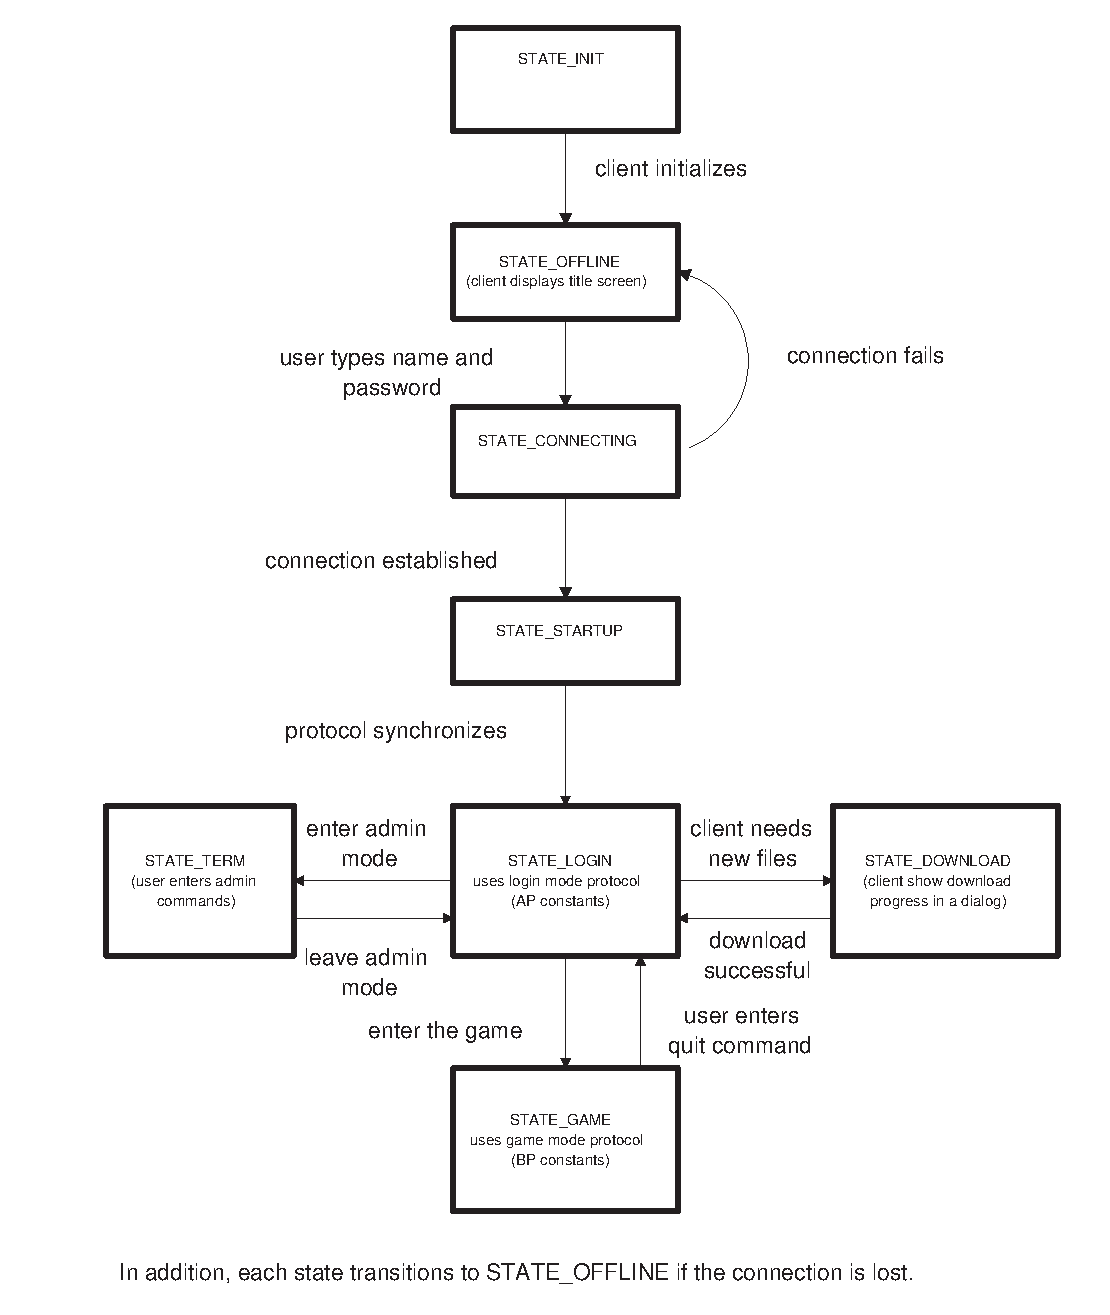
\epsfig{file=cstate1.eps}
\caption{State diagram for the client.}
\label{fig:state1}
\end{figure}

\begin{figure}
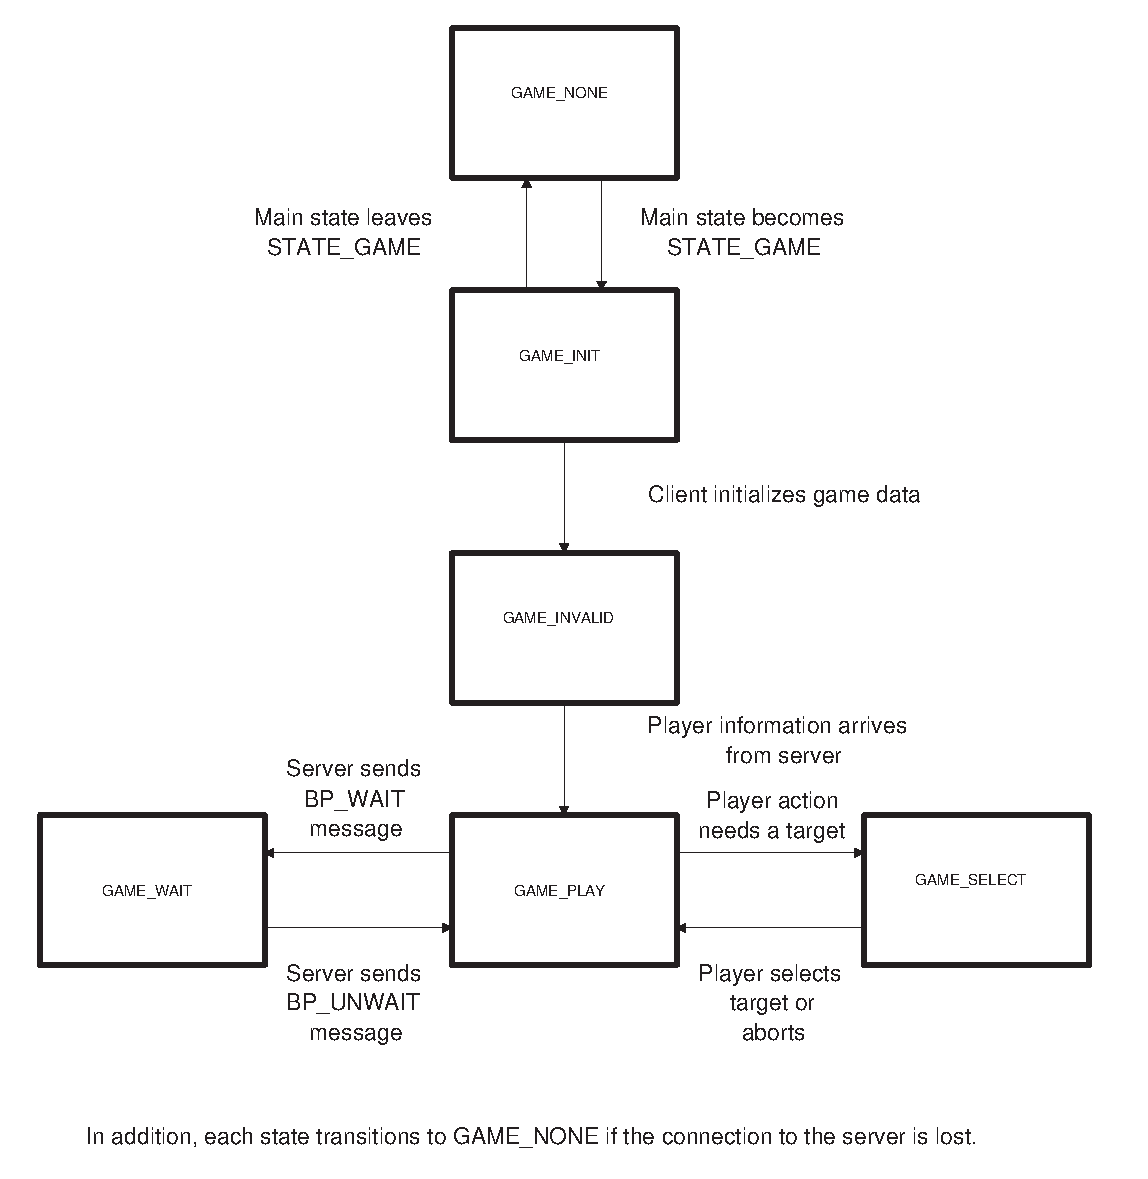
\epsfig{file=cstate2.eps}
\caption{State diagram for the client while it is in the main state
{\tt STATE\_GAME}.}
\label{fig:state2}
\end{figure}

\subsection{Memory usage}

The parts of the client that use the most memory are the frame
buffers, the current room's BSP tree, and the bitmap caches.

The main frame buffer is 452 by 276 pixels, and the larger buffer for
stretched images is twice as large in each direction.  Together, these
total 600 kilobytes of memory, which is allocated when the client
enters the game.

The size of the BSP tree in memory varies widely depending on the size
and complexity of the room.  Current rooms use up to approximately
300-400 kilobytes of memory.  

The client allocates most of free memory to bitmap caches, one for
textures, and one for all other bitmaps.  First the client determines
how much free virtual memory is available, and truncates this amount
at a maximum of 60 megabytes.  Then it estimates the size of the
operating system in memory, and sets aside 75\% of the remaining
amount for the object bitmap cache, and 25\% for the texture cache.
When a bitmap is loaded or accessed, it is added or moved to the front
of the cache's bitmap list; when the cache is full, bitmaps are
removed from the back of the list in least recently used order.

Other pieces that use substantial amounts of memory are the draw list
in the graphics engine, and Windows objects such as fonts, windows,
dialogs, etc.

%%%%%%%%%%%%%%%%%%%%%%%%%%%%%%%%%%%%%%%%%%%%%%%%%%%%%%%%%%%%%%%%%%%%%%%%%
\section{Dynamic updates}

Any part of the client installation can be dynamically updated, even
while the server is still running.  Updates are done via ftp using
Microsoft's Wininet DLL.  The ftp server machine need not be the same
as the game server machine; it is settable in the server's
configuration file.  To help transfers go faster, update files are
compressed with Crusher and decompressed after they are received.

Immediately after logging in, the client sends its version number to
the server.  If the client is out of date, the server tells the client
where to retrieve a new version.  The client then spawns a separate
program called {\tt club}, passing it the ftp server and filename to
download on the command line.  {\tt Club} retrieves the new client
version via ftp, decompresses it, and runs the new version.

The client's INI file contains a sequence number called the {\em
download time}, which identifies the latest data file update the
client has received.  When the client enters the game, it sends its
download time to the server; the server compares the time with the
value in its configuration file.  If the client's download time is
less than the server's configured value, the server sends instructions
on how to update the client's data files.  

On startup, the server reads a text file called {\tt packages.txt},
which contains a line for each action the client should take to update
its download time.  Each line of the file contains a download time, a
filename, and an integer which acts as flags, separated by spaces.
For each download time greater than the client's value, the server
sends these three fields in a message to the client.  The client
interprets the flags field as a particular action to take, and when
this action is complete, it updates the download time in its INI
file.  Assuming that all actions complete successfully, the client
tries to enter the game again; since its download time is now
synchronized to the server's value, it succeeds.

The flags field of a line in {\tt packages.txt} can instruct the
client to download or delete a file, and which directory the file
appears in.  The various flags values allow the client to update files
in any of its subdirectories, so that any data file can be updated.

One particular value of the flags field indicates that the client
should download a new banner advertisement graphic.  Normally, as the
client downloads files, it displays its progress in a dialog box to
the user.  However, to avoid giving the appearance that the game play
is being updated when only advertisements are changing, the client
instead displays a small message dialog as a decoy when all of the
files it needs to update are advertisements.

All of the settings related to updates in the server's configuration
file can be changed dynamically, and the {\tt packages.txt} can also
be edited and reloaded while the server is running.  Thus, any part of
the system can be updated without taking down the server.

%%%%%%%%%%%%%%%%%%%%%%%%%%%%%%%%%%%%%%%%%%%%%%%%%%%%%%%%%%%%%%%%%%%%%%%%%
\section{Security considerations}

Room and resource files are encrypted on client machines, so that
players cannot read or modify them.  Each room file also contains a
checksum that the client verifies when it loads the file, to make sure
it hasn't been modified.  As a final precaution, the client sends this
checksum to the server when it loads the room, and the server verifies
that the client has actually loaded the correct file.  This prevents
players from switching room files.  Other file types, such as
graphics, sound, and music, are stored unencrypted, because players
cannot gain an advantage by modifying them.

User passwords are run through the MD5 one-way hash function algorithm
before they are sent to the server; thus, passwords never appear in
plaintext on the network.  The server stores the hashed passwords in
its account file, so that even the theft of the account file will not
compromise any user accounts.

To prevent players from replaying packets, the protocol contains a
small amount of state.  When the client first connects, the server
sends it seeds for 5 pseudorandom number generators.  Each time the
client sends a message, it includes the output of one of the
generators.  The server verifies that the message contains the correct
pseudorandom number, and both the client and server synchronously
advance their generators.  Any client message that is either repeated
or blocked will be detected by the server.  Currently, when the server
detects such a mismatch, it simply writes the name of the offender to
its log file.

One way the system discourages snooping is by limiting the amount of
game information present on the client.  The world is divided into
rooms, and each client knows only which objects are present in the
same room as the player, as well as the positions and names of these
objects.  The client also has knowledge of the entire map of the room,
and the names of all players who are logged in.  Even armed with all of the
game data present in the client, a player would not have much of an
advantage.  All object data is stored on the server, and only reaches
the client through a restrictive set of messages.

Using the administrator mode, it is possible to gain complete control
over a server.  The client only accepts administrator mode commands
when the server grants it permission; however, it would be possible
for an attacker to modify the client to get it to display
administrator mode.  For this reason, the server verifies each
incoming administrator command, to make sure that its associated
account actually has administrator privileges.  Using administrator
mode thus requires knowledge of an administrator account's password,
or physical access to the server machines.

There are no known security holes in the current scheme.  In order to
cheat, a player would have to reverse the MD5 algorithm, discover the
password to the Crusher encryption scheme or break the scheme,
discover and reproduce the random packet state algorithm, or modify
the client executable.  Even by modifying the client executable, it is
only possible to discover a relatively small amount of information
about the player's local area.
